\icode{N24-MV-MU-L2-261011-001}
\nceeID[6]{2024新课标\Rmnum{2}}{19}
（多选）
位于坐标原点\(O\)的波源在 时开始振动，振动图像如图所示，所形成的简谐横波沿\(x\)轴正方向传播。平衡位置在\(x =\)\, \qty{3.5}{m}处的质点\(P\)开始振动时，波源恰好第2次处于波谷位置，则\paren[]

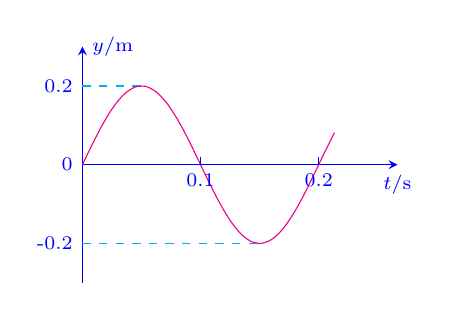
\begin{tikzpicture}[>=stealth,font=\scriptsize]
	\draw[->,blue] (0,0)node[left]{0}--(4,0)node[below]{\(t\)/\qty{}{s}};
	\draw[->,blue] (0,-1.5)--(0,1.5)node[right]{\(y\)/\qty{}{m}};
    \draw[dashed,cyan] (0,1)node[left,blue]{0.2}--(0.75,1);
	\draw[dashed,cyan] (0,-1)node[left,blue]{-0.2}--(2.25,-1);
	\draw[domain=0:3.2,smooth,magenta] plot(\x,{sin(2*pi*\x/3 r)});
	\draw[blue] (1.5,.1)--(1.5,0)node[below,blue]{0.1} (3,.1)--(3,0)node[below,blue]{0.2};
\end{tikzpicture}
\begin{choices}
	\item 波的周期是\qty{0.1}{s}
	\item 波的振幅是\qty{0.2}{m}
	\item 波的传播速度是\qty{10}{m/s}
	\item 平衡位置在\(x =\)\,\qty{4.5}{m}处的质点\(Q\)开始振动时，质点\(P\)处于波峰位置
\end{choices}
\begin{answer}
    BC\qquad 提示：波传播到\(P\)处时间是\(T + \frac{3}{4}T\)
\end{answer}